%\clearpage
%\section{Front-end electronics$^{}$}

The highly integrated front-end (FE) electronics with modular design was developed for a large array of Hamamatsu H8500 and H12700 MAPMTs to minimize the impact of the electronics material on CLAS12 subsystems downstream RICH detector.
An architecture of the readout electronics consists of front-end cards with dedicated Application Specific Integrated Circuit (ASIC) configured, controlled and readout by programmable devices such as Field Programmable Gate Array (FPGA) \cite{RICH_FE}.
The ASIC board is based on the MAROC3  integrated circuit \cite{MAROC} whose excellent single photon capabilities both in analog and binary mode have been confirmed.
%The final design has consists of stacked PCB layers behind each MAPMT sensor (see~Fig.~\ref{fig:feboards}).
%The first layer houses the ASIC front end and ancillary components (e.g. external amplifier) and it is directly connected to the anodes array.
%A second PCB will host the FPGA in charge of configuring, managing and acquiring one or more ASICs and the low voltage and HV bias distribution.
%The use of the JLab SSP as controller and collector of the front-end data provides a strong synergy with the current JLab upgrade activity.
%Data are transmitted on high speed serial (optical) lines minimizing the wiring and therefore the material budget.
%With that sandwich architecture the total photon detection surface will be covered by a fixed number of basic units or tiles made up by two or three sensor each.
%The total spacing for electronics will not exceed 20 cm in depth (including MAPMT and mechanical support).
The three-tiles electronics module with and without 3 H12700 MAPMTs installed is shown on~Fig.~\ref{fig:feboards}.
The performance of MAROC chips was tested and was found suitable for RICH requirements:
\begin{itemize}
	\item 100\% efficiency at 1/3 of single photoelectron signal (50~fC)
	\item time resolution of 1~ns
	\item short deadtime to sustain the trigger rate of 20~kHz
	\item latency of 8~$\mu s$
\end{itemize}

\begin{figure}[htb]
  \centering
  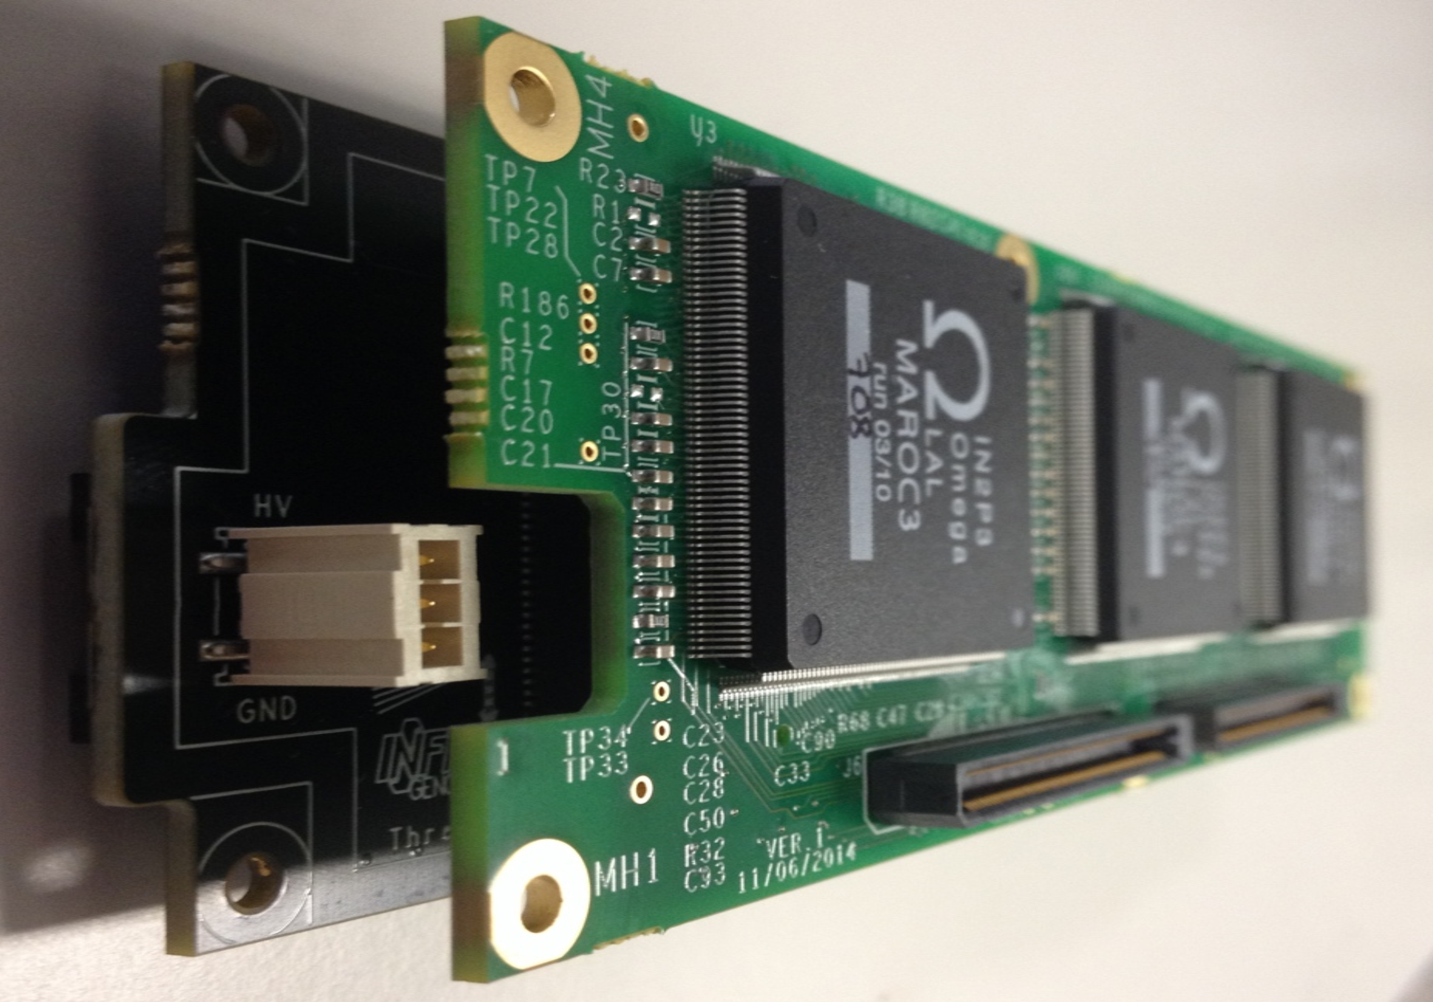
\includegraphics[width=0.8\linewidth]{figures/fe1.pdf}
  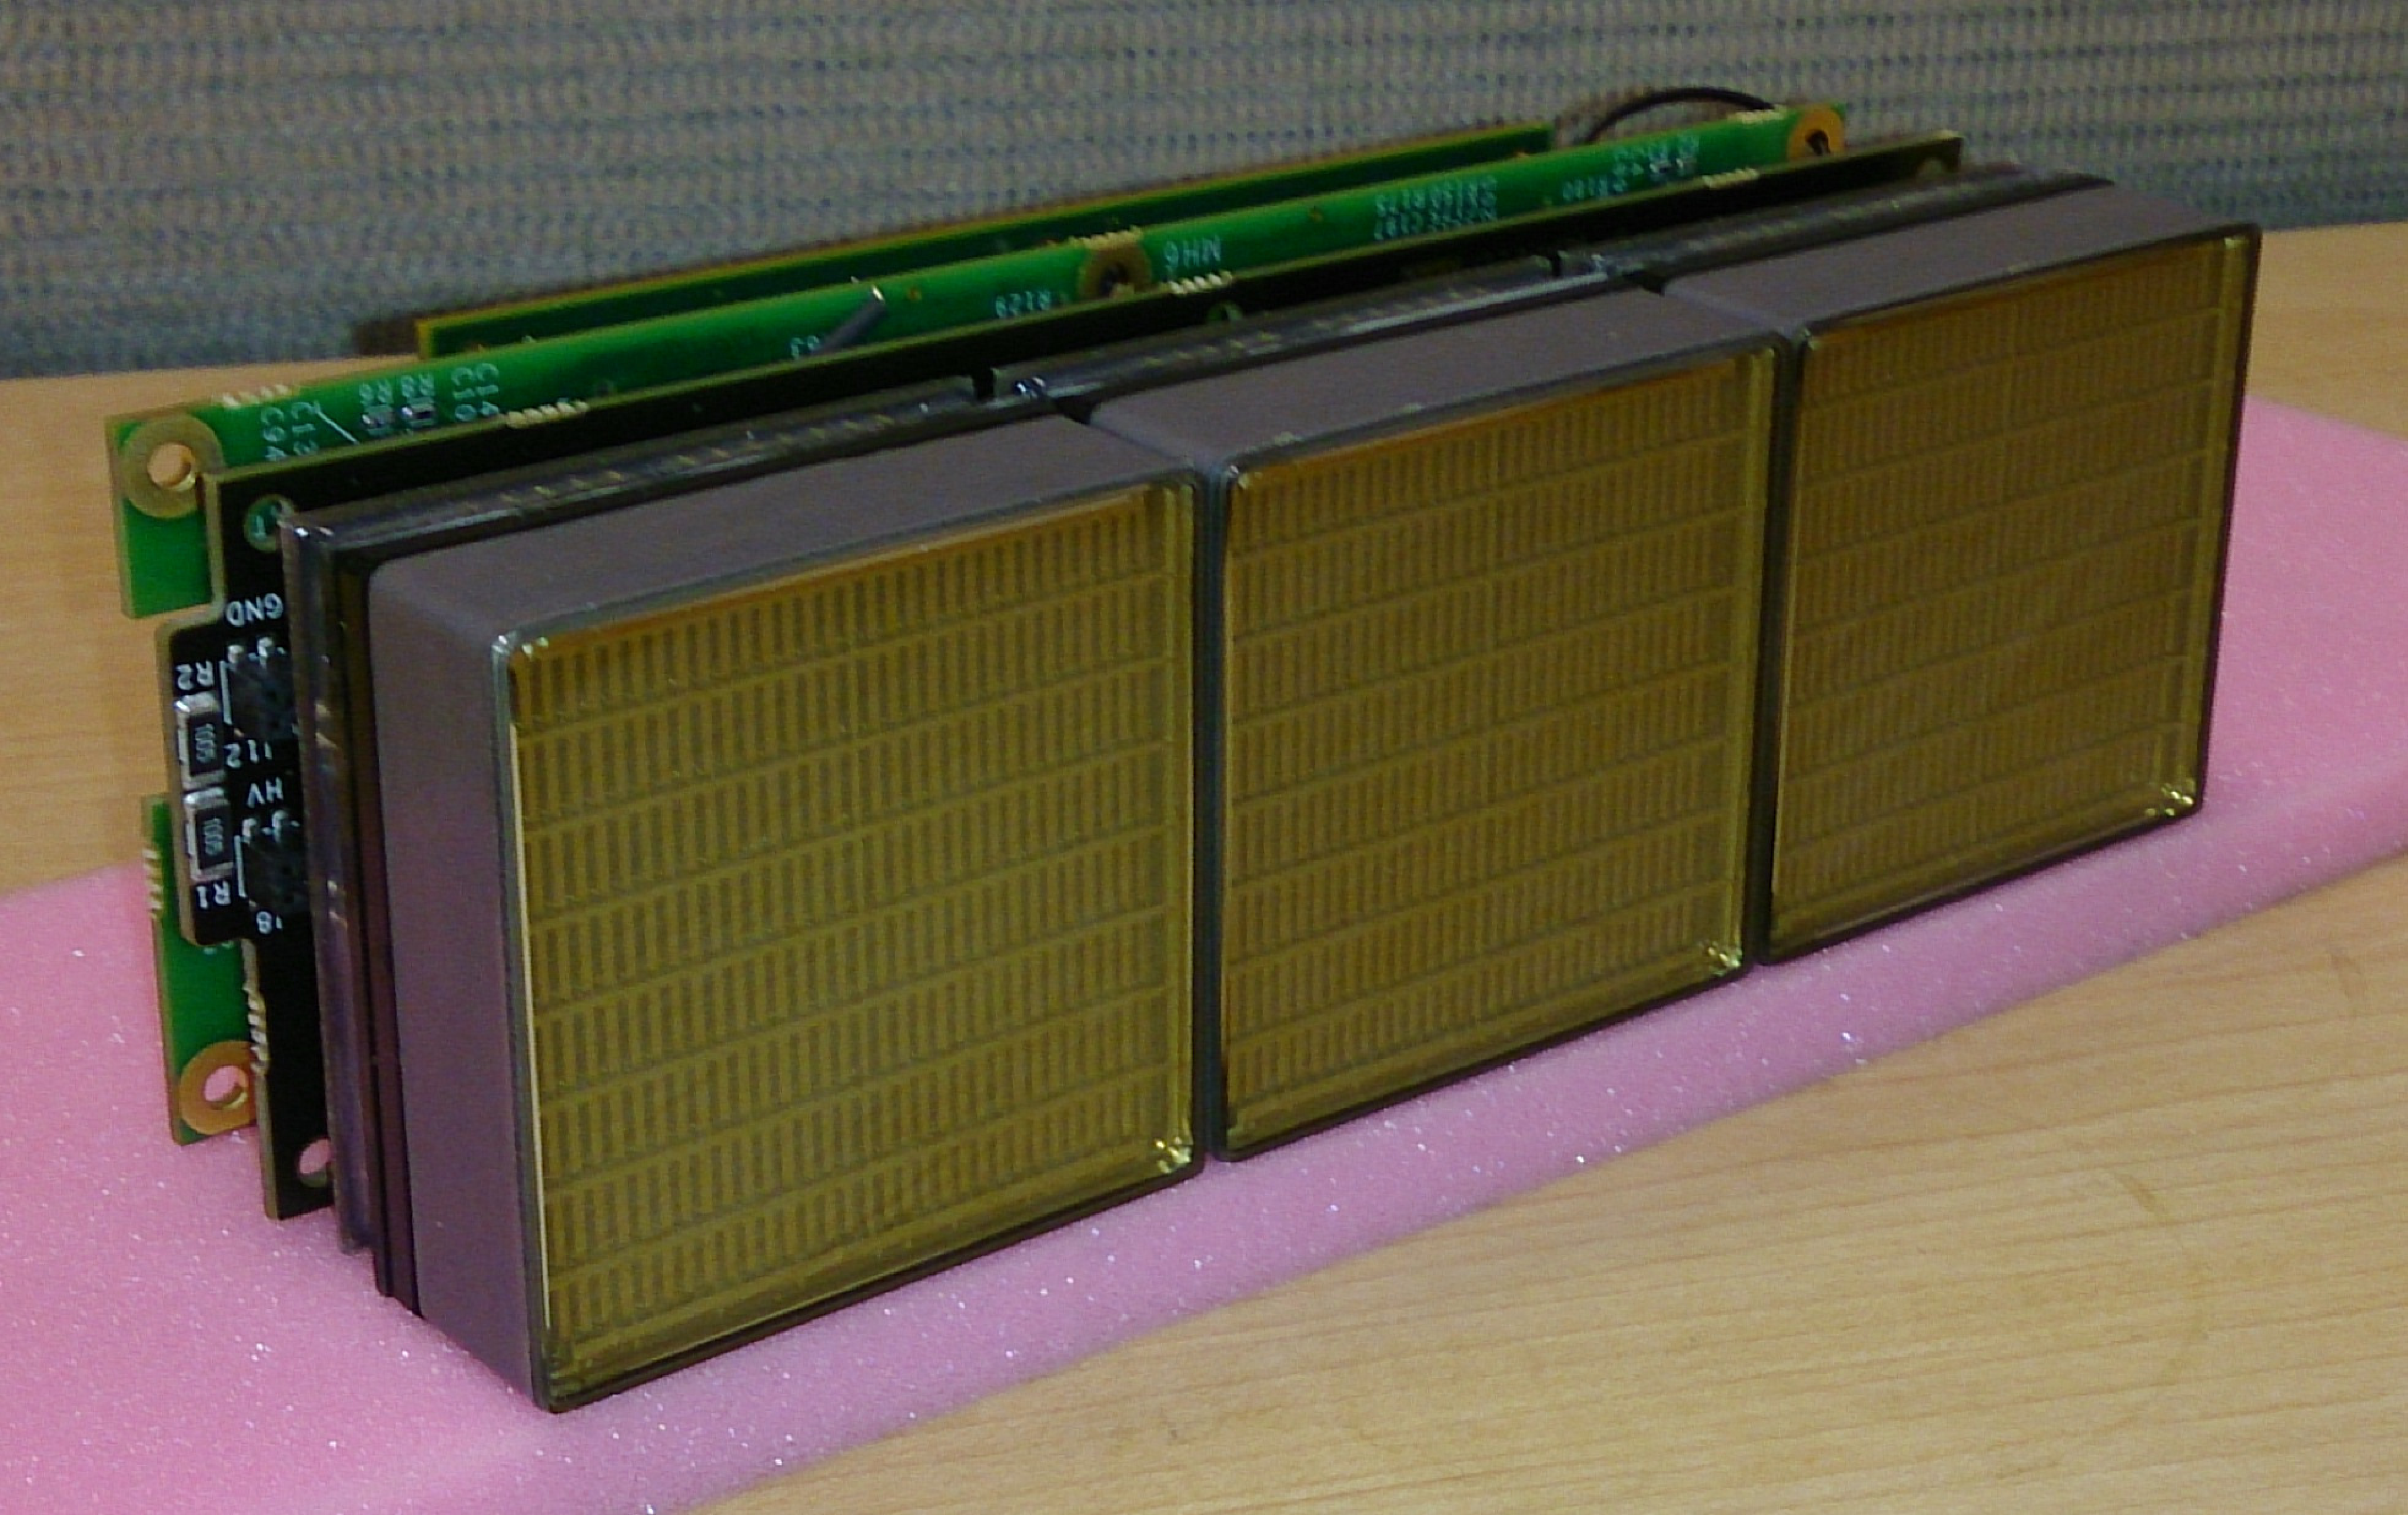
\includegraphics[width=0.8\linewidth]{figures/frontendPMT.pdf}
  \caption{Front-end electronics readout board and mounted MAPMTs.}
  \label{fig:feboards}
\end{figure}

%Each MAROC chip consists of 64 independent channels and is equipped with single channel adjustable preamplifier, configurable signal shaping, slow shaper capable of charge measurements and binary output with fast shaping and adjustable threshold.
%The single channel has a pre-amplification and configurable 8 bit gain correction stage followed by independent binary and analog lines.
%The binary line is digital and most suitable for the RICH application.
%We are planning to analyze the performance of MAROC chip as a function of its threshold and gain.
%Additionally front-end electronics stability and noise will be tested as well.

%The custom modular design as shown on Fig.~\ref{fig:feboards} consists of sandwich architecture where one board hosts the ASIC chips (2 or 3 per board) and another active board hosts the FPGA to manage and configure the ASICs, the third board is a passive adapter for MAPMT sockets.
%The conceptual design of the electronics readout boards was finished in the RICH development phase and currently we have several board implementations available at Jefferson Lab and INFN for final tests.

The measurements of custom front-end electronics together with installed MAPMTs in the RICH Black Box setup were crucial to understand their performance in the RICH detector.
To test and calibrate it multiple tests with internal onboard charge injector, external charge injector and signal generator were performed.
As shown in previous section on Fig.~\ref{fig:MAPMTtest}, RICH MAPMT test setup can house two FE boards inside the black box.
%The focus of the modification was to adapt the test setup in such way that the swap of FE boards would be fast and easy.
%The PCB guidelines were installed inside the black box to ensure easy mounting and dismounting procedure universal for both 2-MAPMT and 3-MAPMT FE modules.
%This requirement exists in light of the future measurements that our group is expected to perform on all FE modules for testing purposes.
%Each FE module is connected to the low voltage power supply to power FPGA and ASIC boards.
The communication between FPGA board and PC is performed using TCP/IP protocol via optical fiber network cable.
%The HV cables, one per each module, supply power for attached MAPMTs.
The Data Acquisition program runs on external PC under Linux OS, configures FPGA and MAROC boards and collects the data through network interface.
%The laser with neutral density filters and light diffuser is installed on a moving platform to allow illumination of individual MAPMTs with different light intensities.
The current setup allows fast evaluation of FE modules with highly automatized procedure which is important because RICH panel consists of 113 tiles with 3-MAPMTs and 23 tiles with 2-MAPMTs FE modules to house 391 MAPMTs.
